\documentclass[a4paper]{article}
\usepackage[utf8]{inputenc}

%=-=-=-=-=-=-=-=-=-=-=-=-=-=-=-=-=-=-=-=-=-=-=-=-=-=-=-=-=-=-=-=-=-=-=-=-=-=-=-=-
% PREAMBLE
%=-=-=-=-=-=-=-=-=-=-=-=-=-=-=-=-=-=-=-=-=-=-=-=-=-=-=-=-=-=-=-=-=-=-=-=-=-=-=-=-

%%%%%%%%%%%%%%%%%%%%%%%%%%%%%%%%%%%%%%%%%%%%%%%%%%%%%%%%%%%%%%%%%%%%%
% Important styling notes
%%
% For now, to include img.jpg in img/path/to/img.jpg, just use:
% path/to/img.jpg - for details see style.tex
%=-=-=-=-=-=-=-=-=-=-=-=-=-=-=-=-=-=-=-=-=-=-=-=-=-=-=-=-=-=-=-=-=-=-=-=-=-=-=-=-
% Packages
%%
%\usepackage{fullpage} % Package to use full page
\usepackage[top=1in,bottom=1in,left=1in,right=1in,heightrounded]{geometry}

\usepackage{parskip}                    % Package to tweak paragraph skipping
\usepackage{amsmath}                    % standard
\usepackage{amssymb}                    % standard - Double R symbol etc.
\usepackage{hyperref}
\usepackage{amsthm}                     % standard - theorem, definition, etc.
\usepackage{multicol}                   % multiple columns for numbering
\usepackage{enumitem}                   % standard - enumerate styles
\usepackage[utf8]{inputenc}
\usepackage{scrextend}                  % indentation
\usepackage{graphicx}                   % standard - add figures
\usepackage{float}                      % standard - figure position, use [H] option
\usepackage{pifont}                     % symbols http://willbenton.com/wb-images/pifont.pdf
                                        % e.g. \ding{51}
\usepackage{gensymb}                    % degree symbol \degree
\usepackage{xcolor}                     % bg color
\hypersetup{
    colorlinks,
    linkcolor={black!50!black},
    citecolor={blue!50!black},
    urlcolor={blue!80!black}
}
\usepackage{framed}                     % bg color
\usepackage[T1]{fontenc}                % small caps
\usepackage{sectsty}                    % headings colour
\usepackage{mathtools}                  % Loads amsmath
\usepackage{amsthm,thmtools,xcolor}     % coloured theorem
\usepackage[toc,page]{appendix}         % reference to appendix
%\usepackage{titlesec}                   % change chapter, section, etc. formats
\usepackage{xifthen}                    % if, else
\usepackage{etoolbox}
% format numbering in theorem, lemma, etc. environment
\AtBeginEnvironment{theorem}{\setlist[enumerate, 1]{font=\upshape,  wide=0.5em, before=\leavevmode}}
\AtBeginEnvironment{lemma}{\setlist[enumerate, 1]{font=\upshape,  wide=0.5em, before=\leavevmode}}
\usepackage[letterspace=150]{microtype} % \textls{<letterspaced text>} % 0 <= letterspace <= 1000, 1000 = M space
\usepackage{letltxmacro}                % renew commands?
\usepackage{minted}                     % package to list code
    % otherwise minted goes off the page
    \setmintedinline{breaklines}
\usepackage{subfig}
\usepackage{eso-pic}                    % title page bg pic
\usepackage{varwidth}
\PassOptionsToPackage{svgnames}{xcolor}
\usepackage{fontawesome}                % \faQuestionCircle
\usepackage{marvosym}                   %\Pointinghand
\usepackage{mdframed}                   % easy outline frames
\usepackage[many]{tcolorbox}            % colour box for theorem styles
\usepackage{array,booktabs,calc} % table figs and text
\usepackage{comment}                    % \begin{comment}
\usepackage{fancyhdr}                   % page headings
\usepackage{mdframed}                   % boxes
\usepackage[backend=biber,sorting=none,style=ieee]{biblatex}
\usepackage{caption}
%%% caption options {
%\DeclareCaptionFont{white}{\color{white}}
\DeclareCaptionFormat{listing}{\colorbox{magenta!30!gray}{\parbox{\textwidth}{#1#2#3}}}
\captionsetup[lstlisting]{format=listing,labelfont={bf,small},textfont=small,skip=-1pt}
%%% }
\addbibresource{bibliography.bib}
\usepackage{url}
\usepackage{textcomp}
\usepackage[makeroom]{cancel}           % crossed symbols - \cancel{}, \bcancel{}, xcancel{}
\usepackage{algorithm}
\usepackage[noend]{algpseudocode}
\usepackage{tikz}
\usetikzlibrary{arrows.meta,positioning,quotes} % arrows and nodes in tikz
\usepackage{marginnote}                 % things in page margin by \marginnote{...}
\usepackage{pgfplots}
\usepackage{pstricks-add,pst-slpe}      % for fancy tikz arrows
%\usepackage{titlesec}                  % title style
\usepackage{lmodern}                    % a font
\usepackage{titletoc}                   % Required for manipulating the table of contents
\usepackage{titlesec}                   % Allows customization of titles
\usepackage{fouriernc}                  % Use the New Century Schoolbook font
\usepackage{booktabs}                   % better tables
\usepackage{stmaryrd }                  % \varoast
\usepackage{listings}                   % code listings
\usepackage{longtable}                  % table across multiple pages
\usepackage{todonotes}                  % TODO bubbles by \todo{...} command
\usepackage{changepage}                 % paragraph margins
\usepackage{tikz}
\usetikzlibrary{calc}
\usepackage{eso-pic}
\usepackage{transparent}
\usepackage[makeroom]{cancel}

%=-=-=-=-=-=-=-=-=-=-=-=-=-=-=-=-=-=-=-=-=-=-=-=-=-=-=-=-=-=-=-=-=-=-=-=-=-=-=-=-
% Colours for various things
%%


\definecolor{shadecolor}{rgb}{1.,0.933,0.96} % bg color, r,g,b <= 1
\definecolor{medium_blue}{RGB}{60,125,190}
\definecolor{dark_blue}{RGB}{25,60,85}
\definecolor{dark_red}{RGB}{77,16,16}
\definecolor{LightPink}{rgb}{0.92.,0.8,0.84} % bg color, r,g,b <= 1
\definecolor{LighterPink}{rgb}{1.,0.94,0.97} % bg color, r,g,b <= 1
\definecolor{LightestPink}{rgb}{1.,0.95,0.99} % bg color, r,g,b <= 1
\definecolor{DarkestPink}{rgb}{0.36, 0.0, 0.18}
\definecolor{DarkerPink}{rgb}{0.41, 0.0, 0.21}
\definecolor{DarkPink}{rgb}{0.55, 0.05, 0.37}
\definecolor{lightestestpink}{RGB}{255,248,252}
\definecolor{codegray}{rgb}{0.5,0.5,0.5}
\definecolor{codegrayblue}{rgb}{0.35,0.35,0.47}



%=-=-=-=-=-=-=-=-=-=-=-=-=-=-=-=-=-=-=-=-=-=-=-=-=-=-=-=-=-=-=-=-=-=-=-=-=-=-=-=-
% Define my own theorem styles
%%

% "base" styles
\declaretheoremstyle[
  headfont=\color{DarkPink}\bfseries,
  bodyfont=\itshape,
]{colored}

\declaretheoremstyle[
  headfont=\color{DarkPink}\bfseries,
  bodyfont=\normalfont,
]{colored_upright}

% theorems (corollaries, etc) themselves, inherit from my style above
% Usage:
% \begin{theorem} \end{theorem}, \begin{lemma} \end{lemma}, ...
\declaretheorem[
	numberwithin=section,
 	style=colored,
	name=\textsc{Theorem},
]{theorem}

\tcolorboxenvironment{theorem}{
  boxrule=0pt,
  boxsep=2pt,
  colback={magenta!25!white},
  colframe=DarkPink,
  enhanced jigsaw, 
  borderline west={2pt}{0pt}{DarkPink},
  sharp corners,
  before skip=5pt,
  after skip=5pt,
  breakable,
  right=0mm % for equations
}

\declaretheorem[
	numberwithin=section,
 	style=colored,
	name=\textsc{Corollary},
]{corollary}

\tcolorboxenvironment{corollary}{
  boxrule=0pt,
  boxsep=1pt,
  colback={magenta!10!white},
  colframe=DarkPink,
  enhanced jigsaw, 
  borderline west={2pt}{0pt}{DarkPink},
  sharp corners,
  before skip=5pt,
  after skip=5pt,
  breakable,
  right=0mm % for equations
}

\declaretheorem[
	numberwithin=section,
	style=colored,
	name=\textsc{Lemma},
]{lemma}

\tcolorboxenvironment{lemma}{
  boxrule=0pt,
  boxsep=1pt,
  colback={magenta!10!white},
  colframe=DarkPink,
  enhanced jigsaw, 
  borderline west={2pt}{0pt}{DarkPink},
  sharp corners,
  before skip=5pt,
  after skip=5pt,
  breakable,
  right=0mm % for equations
}

\declaretheorem[
	numberwithin=section,
	style=colored,
	name=\textsc{Definition},
]{definition}

\tcolorboxenvironment{definition}{
  boxrule=0pt,
  boxsep=1pt,
  colback={magenta!25!white},
  colframe=DarkPink,
  enhanced jigsaw, 
  borderline west={2pt}{0pt}{DarkPink},
  sharp corners,
  before skip=5pt,
  after skip=5pt,
  breakable,
  right=0mm % for equations
}

\declaretheorem[
	numberwithin=section,
  	style=colored,
  	name=\textsc{Example},
]{exmp}

\declaretheorem[
	numberwithin=section,
  	style=colored,
  	name=\textsc{Solution},
]{soln}

%%% code listings
\lstdefinestyle{code1}{
    backgroundcolor=\color{lightestestpink},   
    commentstyle=\color{codegrayblue},
    keywordstyle=\color{DarkerPink},
    numberstyle=\tiny\color{codegray},
    stringstyle=\color{black!40!cyan},
    basicstyle=\small\ttfamily,
    breakatwhitespace=false,
    breaklines=true,        
    captionpos=t,             
    keepspaces=true,        
    numbers=left,           
    numbersep=5pt,
    showspaces=false, 
    showstringspaces=false,
    showtabs=false,
    tabsize=4
}

%%% code listings
\lstdefinestyle{code1}{
    backgroundcolor=\color{lightestestpink},   
    commentstyle=\color{codegrayblue},
    keywordstyle=\color{DarkerPink},
    numberstyle=\tiny\color{codegray},
    stringstyle=\color{black!40!cyan},
    basicstyle=\small\ttfamily,
    breakatwhitespace=false,
    breaklines=true,        
    captionpos=t,             
    keepspaces=true,        
    numbers=left,           
    numbersep=5pt,
    showspaces=false, 
    showstringspaces=false,
    showtabs=false,
    tabsize=4
}


\lstdefinestyle{terminal}{
    backgroundcolor=\color{black!5},   
    commentstyle=\color{codegrayblue},
    keywordstyle=\color{DarkerPink},
    %numberstyle=\tiny\color{codegray},
    stringstyle=\color{black!40!cyan},
    basicstyle=\small\ttfamily,
    numbers=none,
    breakatwhitespace=false,
    breaklines=true,        
    %captionpos=t,             
    keepspaces=true,        
    %numbers=left,           
    %numbersep=5pt,
    showspaces=false, 
    showstringspaces=false,
    showtabs=false,
    tabsize=4
}

\lstset{style=code1}

%=-=-=-=-=-=-=-=-=-=-=-=-=-=-=-=-=-=-=-=-=-=-=-=-=-=-=-=-=-=-=-=-=-=-=-=-=-=-=-=-
% Headers (size, font, colour)
%%

\makeatletter
\renewcommand{\@seccntformat}[1]{\llap{\textcolor{DarkestPink}{\csname the#1\endcsname}\hspace{1em}}}                    
\renewcommand{\section}{\@startsection{section}{1}{\z@}
{-4ex \@plus -1ex \@minus -.4ex}
{1ex \@plus.2ex }
{\normalfont\large\sffamily\bfseries\textcolor{DarkestPink}}}
\renewcommand{\subsection}{\@startsection {subsection}{2}{\z@}
{-3ex \@plus -0.1ex \@minus -.4ex}
{0.5ex \@plus.2ex }
{\normalfont\sffamily\bfseries\textcolor{DarkestPink}}}
\renewcommand{\subsubsection}{\@startsection {subsubsection}{3}{\z@}
{-2ex \@plus -0.1ex \@minus -.2ex}
{.2ex \@plus.2ex }
{\normalfont\small\sffamily\bfseries\textcolor{DarkestPink}}}                        


%=-=-=-=-=-=-=-=-=-=-=-=-=-=-=-=-=-=-=-=-=-=-=-=-=-=-=-=-=-=-=-=-=-=-=-=-=-=-=-=-
% Numberings, counters and spacings
%%
\numberwithin{equation}{section} % section number in eq/s
\setlength{\jot}{7pt} % spacing in split, gathered env/s



%% Custom examples
%% Output - Example 1,2,...
\newcounter{example}
\newenvironment{example}[1][]{\refstepcounter{example}\par\medskip
   \textbf{Example~\theexample. #1} \rmfamily}{\medskip}
%%%%%%%%%%%% End of unused %%%%%%%%%%%%



%=-=-=-=-=-=-=-=-=-=-=-=-=-=-=-=-=-=-=-=-=-=-=-=-=-=-=-=-=-=-=-=-=-=-=-=-=-=-=-=-
% Paths
%%

%=-=-=-=-=-=-=-=-=-=-=-=-=-=-=-=-=-=-=-=-=-=-=-=-=-=-=-=-=-=-=-=-=-=-=-=-=-=-=-=-
% User defined macros (math mode)
%%


% Curly braces under text. Usage: \myunderbrace{upper}{lower}
\newcommand{\myunderbrace}[2]{\mathrlap{\underbrace{\phantom{#1}}_{#2}} #1}
\newcommand{\setR}{\mathbb{R}} % \ouble R
\newcommand{\setRn}{\mathbb{R}^n} %  double R^n
\newcommand{\setN}{\mathbb{N}} % double N
\newcommand{\setZ}{\mathbb{Z}} % double Z
\let\oldemptyset\emptyset
\let\emptyset\varnothing % nice - looking empty set symbol
\newcommand{\fancyN}{\mathcal{N}} % null space
\newcommand{\fancyR}{\mathcal{R}} % range

\newcommand{\ba}{\textbf{a}}
\newcommand{\be}{\textbf{e}}
\newcommand{\bw}{\textbf{w}}
\newcommand{\bx}{\textbf{x}}
\newcommand{\bu}{\textbf{u}}
\newcommand{\bv}{\textbf{v}}
\newcommand{\by}{\textbf{y}}
\newcommand{\bz}{\textbf{z}}
\newcommand{\bb}{\textbf{b}}
\newcommand{\bA}{\textbf{A}}
\newcommand{\bB}{\textbf{B}}
\newcommand{\bC}{\textbf{C}}
\newcommand{\bD}{\textbf{C}}
\newcommand{\bI}{\textbf{I}}
\newcommand{\bM}{\textbf{M}}
\newcommand{\bO}{\textbf{0}}
\newcommand{\bS}{\textbf{S}}
\newcommand{\bX}{\textbf{X}}
\newcommand{\bU}{\textbf{U}}
\newcommand{\bY}{\textbf{Y}}
% double bars as in norm
%\newcommand{\norm}[1] {\left|\left| #1 \right| \right|} 
\newcommand{\norm}[1]{\left\lVert#1\right\rVert}
\renewcommand{\t}{^{\top}}

\newcommand{\mean}[1]{\bar{#1}}
\newcommand{\var}{\sigma^2}

\newcommand{\partdevx}[1]{\frac{\partial #1}{\partial x}}
\newcommand{\partdevt}[1]{\frac{\partial #1}{\partial t}}
\newcommand{\partdevxx}[1]{\frac{\partial #1}{\partial x}}
\newcommand{\partdevxn}[1]{\frac{\partial^n #1}{\partial x^n}}
\newcommand{\partdevy}[1]{\frac{\partial #1}{\partial y}}
\newcommand{\partdevyy}[1]{\frac{\partial #1}{\partial y}}
\newcommand{\partdevyn}[1]{\frac{\partial^n #1}{\partial y^n}}

% text above = symbol
\newcommand{\overeq}[1]{\ensuremath{\stackrel{#1}=}} 
\newcommand{\greatersmaller}{%
  \mathrel{\ooalign{\raisebox{.6ex}{$>$}\cr\raisebox{-.6ex}{$<$}}}
} % greater and smaller symbols on top of each other, same line

%=-=-=-=-=-=-=-=-=-=-=-=-=-=-=-=-=-=-=-=-=-=-=-=-=-=-=-=-=-=-=-=-=-=-=-=-=-=-=-=-
% User defined macros (non math)

\newcommand{\qedblack}{$\hfill\blacksquare$} % black square end of line
\newcommand{\qedwhite}{\hfill \ensuremath{\Box}} % white square end of line
\newcommand{\hquad}{\hskip0.5em\relax}% half quad space
%\newcommand{\TODO}{\textcolor{red}{\bf TODO!}\;}

\newcommand{\TODO}[1][]{%
    \ifthenelse{\equal{#1}{}}{\textcolor{red}{\bf TODO!}\;}{\textcolor{red}{\textbf {TODO:} #1}\; }%
}
\newcommand{\B}[1]{\textbf{\textup{#1}}} % bold and upright
\renewcommand{\labelitemi}{\scriptsize$\textcolor{DarkPink}{\blacksquare}$} % itemize - squares instead of bullets
\newcommand{\emphasis}[1]{\textls{#1}}

\LetLtxMacro{\originaleqref}{\eqref}
\renewcommand{\eqref}{Eq.~\originaleqref}
\renewcommand*{\eqref}[1]{Eq.~\originaleqref{#1}}





% background images
%%%%%%%
\newcommand\BackgroundPic{%
\put(0,0){%
\parbox[b][\paperheight]{\paperwidth}{%
\vfill
%\centering
\includegraphics[width=0.125\paperwidth,height=\paperheight,%
]{img/background_02.png}% use ,keepaspectratio
\vfill
}}}
%%%%%%%
% end of background image
%%%%%%%%%%%%%% my own frame
\newmdenv[topline=false,bottomline=false]{leftrightbox}
%%%%%%%%%%%%% end
%%%%%%%%%%%%% my own comment
\newcommand{\mycomment}[1]{\begin{leftrightbox}\Pointinghand~\textbf{Comment:}~#1 \end{leftrightbox}}
%%%%%%%%%%%%% end
% my custom note https://tex.stackexchange.com/questions/301993/create-custom-note-environment-with-tcolorbox
\newmdenv[
    topline=false,
    bottomline=false,
    rightline=false,
    innerrightmargin=0pt
]{siderule}
\newenvironment{mynote}%
    {\begin{siderule}\textbf{\Pointinghand~Note:}}
    {\end{siderule}}
    
\newenvironment{myquote}%
    {\begin{adjustwidth}{0.4cm}{0.4cm}\faQuoteLeft\ \itshape}
    { \hfill \faQuoteRight  \end{adjustwidth}}
%%%%%%%%%%%%% my own box
\newcommand{\boxone}[1]{\begin{tcolorbox}[colback = LighterPink,colframe=LightPink]
#1
\end{tcolorbox}}
\newcommand{\boxsimple}[1]{\begin{tcolorbox}[
	colback = white,
	colframe=black!70,
	coltitle = black!20,
	title    = {Problem},]
#1
\end{tcolorbox}}
%%%%%%%%%%%%% end

\newcommand{\bigtitle}[1]{\LARGE\textsc{{\textbf{#1}}}\normalsize\vspace{0.25cm}}

\let\oldemptyset\emptyset
\let\emptyset\varnothing
%algorithmic
\algdef{SE}[DOWHILE]{Do}{doWhile}{\algorithmicdo}[1]{\algorithmicwhile\ #1}%

%%% otherwise minted goes off the page
\setmintedinline{breaklines}




\begin{document}
%=-=-=-=-=-=-=-=-=-=-=-=-=-=-=-=-=-=-=-=-=-=-=-=-=-=-=-=-=-=-=-=-=-=-=-=-=-=-=-=-
% GLOBAL STYLES (DOCUMENT SCOPE)
%=-=-=-=-=-=-=-=-=-=-=-=-=-=-=-=-=-=-=-=-=-=-=-=-=-=-=-=-=-=-=-=-=-=-=-=-=-=-=-=-
% caption: Figure 1 -> <bold> Fig. 1 </bold>
\captionsetup[figure]{labelfont={bf},labelformat={default},labelsep=period,name={Fig.}}


%=-=-=-=-=-=-=-=-=-=-=-=-=-=-=-=-=-=-=-=-=-=-=-=-=-=-=-=-=-=-=-=-=-=-=-=-=-=-=-=-
% TITLE PAGE
%=-=-=-=-=-=-=-=-=-=-=-=-=-=-=-=-=-=-=-=-=-=-=-=-=-=-=-=-=-=-=-=-=-=-=-=-=-=-=-=-
%%%%%%%%%%%%%%%%%%%%%%%%%%%%%%%%%%%%%%%%%
% Formal Book Title Page
% LaTeX Template
% Version 2.0 (23/7/17)
%
% This template was downloaded from:
% http://www.LaTeXTemplates.com
%
% Original author:
% Peter Wilson (herries.press@earthlink.net) with modifications by:
% Vel (vel@latextemplates.com)
%
% License:
% CC BY-NC-SA 3.0 (http://creativecommons.org/licenses/by-nc-sa/3.0/)
% 
% This template can be used in one of two ways:
%
% 1) Content can be added at the end of this file just before the \end{document}
% to use this title page as the starting point for your document.
%
% 2) Alternatively, if you already have a document which you wish to add this
% title page to, copy everything between the \begin{document} and
% \end{document} and paste it where you would like the title page in your
% document. You will then need to insert the packages and document 
% configurations into your document carefully making sure you are not loading
% the same package twice and that there are no clashes.
%
%%%%%%%%%%%%%%%%%%%%%%%%%%%%%%%%%%%%%%%%%

%----------------------------------------------------------------------------------------
%	PACKAGES AND OTHER DOCUMENT CONFIGURATIONS
%----------------------------------------------------------------------------------------



%----------------------------------------------------------------------------------------
%	TITLE PAGE
%----------------------------------------------------------------------------------------



\begin{titlepage} % Suppresses headers and footers on the title page

	%------------------------------------------------
	%	Border decorations
	%------------------------------------------------
    \AddToShipoutPictureBG*{
        \begin{tikzpicture}[overlay,remember picture]
            \draw[line width=10pt]
                ($ (current page.north west) + (4pt,-4pt) $)
                rectangle
                ($ (current page.south east) + (4pt,4pt) $);
            \draw[line width=10pt]
                ($ (current page.north west) + (4pt,-4pt) $)
                rectangle
                ($ (current page.south east) + (-4pt,4pt) $);
        \end{tikzpicture}
        \AtTextUpperLeft{%
            \put(185,12){
                \parbox[b][\paperheight]{\paperwidth}{% parbox
            
                    \centering
                    {\transparent{1.0}
                    \setlength{\fboxsep}{0pt}%
                    \setlength{\fboxrule}{2pt}%
                    \fbox{                                
                        \includegraphics[keepaspectratio=false,width=50pt,height=50pt]{img/title/corner.png}
                        }
                    } % transparent
                } % parbox
            } % put
        } % AtTextUpperLeft
        
        \AtTextUpperLeft{%
            \put(185,-762){
                \parbox[b][\paperheight]{\paperwidth}{% parbox
            
                    \centering
                    {\transparent{1.0}
                    \setlength{\fboxsep}{0pt}%
                    \setlength{\fboxrule}{2pt}%
                    \fbox{                                
                        \includegraphics[keepaspectratio=false,width=50pt,height=50pt]{img/title/corner.png}
                        }
                    } % transparent
                } % parbox
            } % put
        } % AtTextUpperLeft
        
         \AtTextUpperLeft{%
            \put(-338,-762){
                \parbox[b][\paperheight]{\paperwidth}{% parbox
            
                    \centering
                    {\transparent{1.0}
                    \setlength{\fboxsep}{0pt}%
                    \setlength{\fboxrule}{2pt}%
                    \fbox{                                
                        \includegraphics[keepaspectratio=false,width=50pt,height=50pt]{img/title/corner.png}
                        }
                    } % transparent
                } % parbox
            } % put
        } % AtTextUpperLeft
        
        \AtTextUpperLeft{%
            \put(-338,12){
                \parbox[b][\paperheight]{\paperwidth}{% parbox
            
                    \centering
                    {\transparent{1.0}
                    \setlength{\fboxsep}{0pt}%
                    \setlength{\fboxrule}{2pt}%
                    \fbox{                                
                        \includegraphics[keepaspectratio=false,width=50pt,height=50pt]{img/title/corner.png}
                        }
                    } % transparent
                } % parbox
            } % put
        } % AtTextUpperLeft
    } %AddToShipoutPictureBG
    
    
   	%------------------------------------------------
	%	Text alignment
	%------------------------------------------------
	\centering % Centre everything on the title page
	
	\scshape % Use small caps for all text on the title page
	
	\vspace*{\baselineskip} % White space at the top of the page
	
	%------------------------------------------------
	%	Title
	%------------------------------------------------
	
	\rule{\textwidth}{1.6pt}\vspace*{-\baselineskip}\vspace*{2pt} % Thick horizontal rule
	\rule{\textwidth}{0.4pt} % Thin horizontal rule
	
	\vspace{0.75\baselineskip} % Whitespace above the title
	
	{\LARGE NOTES ON\\ \Large 3D GEOMETRY FOR COMPUTER VISION\\ \Large AND SLAM} % Title
	
	\vspace{0.75\baselineskip} % Whitespace below the title
	
	\rule{\textwidth}{0.4pt}\vspace*{-\baselineskip}\vspace{3.2pt} % Thin horizontal rule
	\rule{\textwidth}{1.6pt} % Thick horizontal rule
	
	\vspace{2\baselineskip} % Whitespace after the title block
	
	%------------------------------------------------
	%	Subtitle
	%------------------------------------------------
	Contents
	
	\vspace*{3\baselineskip} % Whitespace under the subtitle
	
	Projective Geometry\\
	Image Rectification\\
	SLAM
	
	\vspace*{3\baselineskip} % Whitespace under the subtitle
	
	%------------------------------------------------
	%	Editor(s)
	%------------------------------------------------
	
	By
	
	\vspace{0.5\baselineskip} % Whitespace before the editors
	
	{\normalfont \Large \mintinline{latex}{0xLeo} (\url{github.com/0xleo}) \\} % Editor list
	
	\vspace{0.5\baselineskip} % Whitespace below the editor list
	
	%\textit{The University of California \\ Berkeley} % Editor affiliation
	
	\vfill % Whitespace between editor names and publisher logo
	
	%------------------------------------------------
	%	Publisher
	%------------------------------------------------
	
	
	\vspace{0.3\baselineskip} % Whitespace under the publisher logo
	
	\today % Date
	
	{DRAFT X.YY} % Draft version
	{\\Missing: \ldots}

\end{titlepage}

%----------------------------------------------------------------------------------------
%\maketitle



%=-=-=-=-=-=-=-=-=-=-=-=-=-=-=-=-=-=-=-=-=-=-=-=-=-=-=-=-=-=-=-=-=-=-=-=-=-=-=-=-
% MAIN DOCUMENT
%=-=-=-=-=-=-=-=-=-=-=-=-=-=-=-=-=-=-=-=-=-=-=-=-=-=-=-=-=-=-=-=-=-=-=-=-=-=-=-=-
\newpage
\tableofcontents
\newpage



%------------------------------ New section ------------------------------%
\section{Multiclass and Binary Logistic Regression Activation and Error Functions}

This is a template that includes all packages and styles I need for writing notes.


\subsection{Perceptron binary classification drawbacks}

So far, we've seen the perceptron, which was trying to classify a set of data points  $\bx^{(1)},\ \ldots,\ \bx^{(n)}$ in two classes -- positive and negative using the prediction formula $\hat{y} = f(w_1x_1 + w_2x_2 + b)$, where $f$ is the step function. For each misclassified point, it would adjust the weights and bias $w_1,\ w_2,\ b$ based on the coordinates of the point. An error function wasn't defined but simply measuring the number of misclassified points is not good enough for the job.

\subsection{A better activation function -- the sigmoid}

The closer to $0$ the argument of the step function is, i.e. $\textbf{w}\cdot \bx$ the more uncertain we are about which class it belongs to and instead of assigning it a probability of $1$ or $0$, we assign it a continuous value from $0$ to $1$. A good probability (activation) function that is symmetric around $0$ and scales the output from $0$ to $1$ is the sigmoid function. For values $x\rightarrow -\infty$, its value is close to 0, for values close to $0$ its value is $0.5$ and for values $x\rightarrow \infty$, its value is close to 1.

\begin{definition}[sigmoid function] 
The \emphasis{sigmoid activation function} is continuous and differentiable and defined as
\begin{equation}
    \sigma(x) = \frac{1}{1 + e^{-x}}
\end{equation}
\end{definition}
\begin{figure}[H]
    \centering
    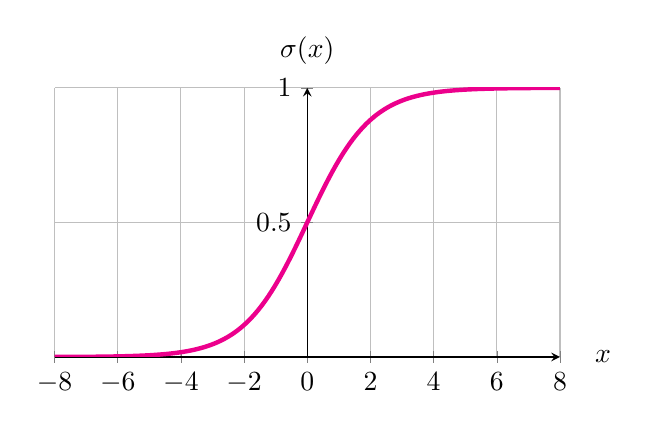
\begin{tikzpicture}
    \begin{axis}%
    [
        height=5cm,
        width=8cm,
        grid=major,     
        xmin=-8,
        xmax=8,
        axis x line=bottom,
        ytick={0,.5,1},
        ymax=1,
        axis y line=middle,
        xlabel=$x$,
        ylabel=$\sigma(x)$,
        every axis x label/.style={
            at={(ticklabel* cs:1.05)},
            anchor=west
        },
        every axis y label/.style={
            at={(ticklabel* cs:1.05)},
            anchor=south,
        },
    ]
        \addplot%
        [
            color=magenta,
            ultra thick,
            mark=none,
            samples=150,
            domain=-8:8,
        ]
        (x,{1/(1+exp(-x))});
    \end{axis}
\end{tikzpicture}
    \caption{The sigmoid function.}
\end{figure}
Suppose in the following figure that we classify some points based on their colour being blue/ not blue. Then $\hat{y}=f(\textbf{w}\cdot \bx + b)=1$ for blue points that are certainly and $\hat{y}=0$ for points that are certainly red. Each point in the plane will have a weighed sum $\textbf{w}\cdot \bx + b$, based on the weights and bias of the line. Using the sigmoid as the perceptron activation function, each point will be assigned a value $\in[0,1]$ instead of 0 or $1$.
\begin{figure}[H]
    \centering
    \includegraphics[height=5cm]{img/sigmoid_of_perc.PNG}
    \caption{The probability of being blue of each point in the $x_1,\ x_2$ space. Note that for each line the probability is the same.}
    \label{fig:my_label}
\end{figure}

\begin{figure}[H]
    \centering
    \includegraphics[height=4.75cm]{img/blue_red_example_valsPNG.PNG}
    \caption{Using the sigmoid, the perceptron outputs continuous values. Those on the black line are $0.5$.}
\end{figure}
So far, the sigmoid-based perceptron outputs for each point a probility that it belongs to the blue class $P(\textup(blue))$ and one that doesn't, $P(\textup{not \;\; blue})$ such that $P(\textup{blue}) + P(\textup{not \;\; blue})=1$.



\subsubsection{Multi-class classification}

\subsubsection{One-hot encoding}

The first difference between binary and multiclass classification is that the label $y$ doe not only take the values $0$ and $1$, but it should take $K$ different values, where $K$ is the number of classes. Let's say we have some data $(\bx^{(1)},\ y^{(1)}), \ldots, \ (\bx^{(n)},\ y^{(n)})$. 

% ref https://www.cs.toronto.edu/~guerzhoy/321/lec/W04/onehot.pdf
Suppose, for instance, that the data represent the output of an image classifier, and we have $K=3$ classes. 


Sigmoid doesn't work for more than two classes. In this section, we study softmax regression, which generalises logistic regression
to classification problems where the class label $y$ can take on more than two possible values. Suppose we have a set of $n$ inputs $\bx^{(1)},\ \ldots, \ \bx^{(n)}$ and we want to classify them in $K=3$ classes -- $y^{(i)} \in \{``person'',\ ``hamster'',\ ``capybara'' \}$. 

One way to encode them would be $y^{(i)} \in \{1,\ 2,\ 3\}$. However, that would imply that ``hamster'' is the average of ``person'' and ``capybara'' and wouldn't allow linear regression to run correctly. When classifying, there shouldn't be the concept of distance between classes. A better way to encode them would be using an one-hot vector for each class, particularly:
\begin{gather*}
\textup{person} \Rightarrow \by^{(1)} = \begin{bmatrix} 1 & 0 & 0\end{bmatrix}^\top\\
\textup{hamster} \Rightarrow \by^{(2)} = \begin{bmatrix} 0 & 1 & 0\end{bmatrix}^\top\\
\textup{capybara} \Rightarrow \by^{(3)} = \begin{bmatrix} 0 & 0 & 1\end{bmatrix}^\top\\
\end{gather*}
% ref http://www.it.uu.se/edu/course/homepage/sml/literature/lecture_notes.pdf
\begin{definition}[one-hot encoding] If the number of classes is $K$, and a data point $\bx^{(i)}$  belongs in the $i$-th class, then using \emphasis{one-hot encoding} it is represented by:
\begin{equation}
    \by^{(i)} = \underbrace{\begin{bmatrix}0 & \ldots & 0 & \underbrace{1}_{\textup{index} \;\; i} &0 & \ldots  & 0\end{bmatrix}^\top}_{K \times 1}
\end{equation}
\end{definition}


\subsubsection{Activation function for multiclass model}

The sigmoid activation only works for the binary model. In this section, we extend it for more than 2 classes, e.g. $K$ classes. Once again, for each input data point $\bx$ we need to compute the ``pre-activation scores'' 
\begin{align*}
    z^{(1)} &= \bx \cdot \bw^{(1)} + b^{(1)} = \bx ^\top \bw^{(1)} + b^{(1)}  \\
    z^{(2)} &= \bx ^\top \bw^{(2)} + b^{(2)}  \\
    \ldots\\
    z^{(K)} &= \bx ^\top \bw^{(K)} + b^{(K)} \\
\end{align*}
Each score is obtained by binary linear regression with weights $\bw$. We now want one classifier such that:
\begin{enumerate}
    \item Each output $\hat{\textbf{y}}^k$  is non-negative.
    \item The sum of $\hat{\textbf{y}}^k$ over all $K$ classes is $1$.
\end{enumerate}
The \emphasis{softmax} function meets both of those requirements.
\begin{definition}[softmax function] Given a classifier of $K$ classes, the softmax function outputs a $K\times 1$ vector where entry $j$ has the value
\begin{equation}
    softmax(\bz^{(j)})=\hat{\by}^{(j)}=\frac{\exp(\bz_j)}{\sum \limits _{j=1}^{j=K}{\exp(\bz_j)}}
\end{equation}
\end{definition}
\marginnote{Often we denote the softmax function as $h$ as it represents the hypothesis given the weights and biases $\bw , \bb$.} The softmax meets all the requirements of a probability function therefore the softmax of pre-activation score $\bz ^ {(j)}$ represents the likelihood of the measurement $\textbf{x}$ belonging in each class $y=j$.
\begin{corollary}
% ref http://www.it.uu.se/edu/course/homepage/sml/literature/lecture_notes.pdf
The probabity of the data point $\bx^{(i)} $ belonging  in each class $1,\ 2, \ldots, \ K$ is given by the softmax function:
\begin{equation}
    \begin{bmatrix}
        P(1\ |\ \bx^{(i)}) \\
        P(2\ |\ \bx^{(i)}) \\
        \ldots \\
        P(K\ |\ \bx^{(i)}) \\
    \end{bmatrix} 
    = softmax(\bz^{(i)}), \quad \bz^{(i)} =
    \begin{bmatrix}
    \trans{\bw}_1 \bx^{(i)} + b_1 \\
    \trans{\bw}_2 \bx^{(i)} + b_2 \\
    \ldots \\
    \trans{\bw}_K \bx^{(i)} + b_K \\
    \end{bmatrix}
\end{equation}
Equivalently,
\begin{equation}
    P(k \ | \ \bx^{(i)}) = \frac{\exp(\trans{\bw}_k \bx^{(i)} + b_k)}
    {\sum_{j=1}^{j=K}{\exp(\trans{\bw}_j \bx^{(i)} + b_j})}
\end{equation}
\end{corollary}
$\sum_{j=1}^{j=K}{\exp(\trans{\bw}_j \bx^{(i)} + b_j})$ is just the normalisation term so requirement (2) can be fulfiled. To summarise, the order of operation before the softmax of each class is computed is shown below.
\begin{figure}[H]
    \centering
    \includegraphics[height=4.5cm]{img/softmax_neural_net.PNG}
    \caption{The steps of softmax computation.}
\end{figure}
%\marginnote{y }
% better example: https://www.quora.com/What-is-the-intuition-behind-SoftMax-function
\begin{exmp}
Let $m=2$ be the number of features, $K=3$ the classes and $\bx=\begin{bmatrix}1 & 1 \end{bmatrix}^\top$ and the weights of each class be $\bw^{(1)}=\begin{bmatrix}-2.5 & -1 \end{bmatrix}, \; \bw^{(2)}=\begin{bmatrix}1 & 2 \end{bmatrix}, \; \bw^{(3)}=\begin{bmatrix}1 & 0 \end{bmatrix}$. Which class does $\bx$ belong to?
\end{exmp}
\begin{soln}
Find the $\bz$ vector.
\begin{align*}
\bz^{(1)} &= {\bw^{(1)}}^\top \bx = 
\begin{bmatrix} -2.5 & -1\end{bmatrix}\begin{bmatrix} -1 \\ 1\end{bmatrix} = 1.5 \\
\bz^{(2)} &= {\bw^{(2)}}^\top \bx = 1 \\
\bz^{(3)} &= {\bw^{(3)}}^\top \bx = -1
\end{align*}
Using the softmax for each score we can find the prediction vector:
\[
\hat{\by} = \begin{bmatrix}.592 \\ .359 \\ .049 \end{bmatrix}
\]
The prediction with highest probability is for class 1. \qedblack
\end{soln}
% ref http://www.sfs.uni-tuebingen.de/~ddekok/dl4nlp/softmax-regression.pdf
\begin{corollary}
For $K=2$ classes, the softmax and sigmoid functions for classification are equivalent.
\end{corollary}
In the next section, we examine how to measure the correctness of the whole model, i.e. how $\bw^{(1)}, \ \ldots, \ \bw^{(K)}$ have ben tuned such that $\hat{\by}$ is as close as possible to the ground truth $\by$.


\subsection{Logistic regression error functions}

\subsubsection{Coming up with an error function -- intuition}

Let's consider the binary logistic regression problem again. Suppose we want to classify points as ``blue'' and ``red'' and we have the linear classifiers in the Fig. \ref{fig:red_blue_points_est}. Note that in Fig. \ref{fig:red_blue_points_est}, red points are \textit{actually} red and so are the blue ($y^{(i)}=1$ for blue, $y^{(i)}=0$ for red). The colour gradient illustrates what the classifier has predicted for the points above or below it, i.e. the estimated probability of the point being blue $\hat{y}^{(i)} = P\left(y^{(i)}\ | \ \bx^{(i)}\right)  \in [0,1]$. Of course along the line we have $\hat{y}^{(i)}=0.5$.

\begin{figure}[H]
    \centering
    \includegraphics[height=4cm]{img/2_linear_models_prob.PNG}
    \caption{Two linear binary classification models. The colour of the points shows what they \textit{actually} are and the colour gradient what the predictor has \textit{estimated}.}
    \label{fig:red_blue_points_est}
\end{figure}

As shown in Fig. \ref{fig:red_blue_points_est}, a good way to measure the performance of each classifier w.r.t. the actual label is by measuring the total probability -- $0.6\cdot0.2\cdot0.1\cdot0.7=0.0084$ and $0.7\cdot0.9\cdot0.8\cdot0.6=0.3024$ for the first and second model. The higher the total probability, the better the predictions. What's an analytical expression for this product?

The model outputs a value between 0 and 1, with 1 for points predicted as ``blue'' and 0 those as ``red''. For each term in the product, given that it's a blue, i.e. $y^{(i)}=1$, we want $y^{(i)} \ \hat{y}^{(i)}$ to be large. Given that it's red, i.e. $y^{(i)}=0$, we want $\left( 1 - y^{(i)} \right)\  \left( 1 - \hat{y}^{(i)}\right)$ to be large. Thus, the larger the product, the better the predictions. 


\subsubsection{Binary regression log loss cost function}

When designing an error function, we want it to fulfil the following requirements.
\begin{itemize}
    \item To be large when the prediction $\hat{y}$ is different from the actual label $y$.
    \item To be convex so that it can be optimised.
\end{itemize}

As motivated in the previous section, we want to find model weights and bias (denote them all $w$ for convenience) that maximise the probability of the actual labels $y^{(i)}$ given the input $\bx^{(i)}$:
% ref https://gluon.mxnet.io/chapter02_supervised-learning/logistic-regression-gluon.html
\begin{equation*}
    w = \arg \ \underset{w}{\mathop{\max }}\,{{P}_{w}}\left( \left( y^{(1)},\ \ldots,\ y^{(n)} \right)\ 
    \left| \ \bx^{(1)},\ \ldots,\ \bx^{(n)}  \right. \right)
\end{equation*}
Since each label $y^{(i)}$ is independent of the others as it depends only on the features of the corresponding example, this can expanded as products:
\[
    w = \arg \ \underset{w}{\mathop{\max }}\,
    P_{w}\left( y^{(i)} \ \left| \ \bx^{(i)} \right. \right)
    P_{w}\left( y^{(2)} \ \left| \ \bx^{(2)} \right. \right)
    \ldots
    P_{w}\left( y^{(n)} \ \left| \ \bx^{(n)} \right. \right)
\]
This seems to be a good loss function but as shown in the previous section, especially for large numbers of data points, this may output a probability very close to 0, which can be numerically unstable. It's easier to work with sums, i.e. take the $\log$ of the product:
\[
    w = \arg \ \underset{w}{\mathop{\max }}\, 
    \left (
    \log \ P_w\left( y^{(1)} \ \left| \ \bx^{(1)} \right. \right)+
    \log \ P_w\left( y^{(2)} \ \left| \ \bx^{(2)} \right. \right)+
    \ldots+
    \log \ P_w\left( y^{(n)} \ \left| \ \bx^{(n)} \right. \right)
    \right)
\]
The part inside the $\max$ is the \emphasis{objective function}, or cost function. Because we usually want to minimise it, we flip the sign behind each term so:
\[
    w = \arg \ \underset{w}{\mathop{\min }}\, 
    \left(
    -\sum \limits _{i=1} ^{n} {\log \ P_w\left( y^{(i)} \ \left| \ \bx^{(i)} \right. \right)}
    \right)
    \tag{1}
\]
As established in the previous section $y^{(i)}=1$ if $\bx^{(i)}$ belongs to the ``positive'' class, therefore then we have $P_w\left( y^{(i)} \ \left| \ \bx^{(i)} \right. \right) = \hat{y}^{(i)}$. If $\bx^{(i)}$ belongs to the ``negative'' class, then $y^{(i)}=0$ therefore $P_w\left( y^{(i)} \ \left| \ \bx^{(i)} \right. \right) = 1 - \hat{y}^{(i)}$, i.e.
\[
P_w\left( y^{(i)} \ \left| \ \bx^{(i)} \right. \right)= \left\{
\begin{array}{ll}
      \hat{y}^{(i)} & y^{(i)}=1 \\
      1-\hat{y}^{(i)} & y^{(i)}=0\\
\end{array} 
\right. 
\]
This can be written in a more compact form as
\[
P_w\left( y^{(i)} \ \left| \ \bx^{(i)} \right. \right)=
(\hat{y}^{(i)})^{y^{(i)}} (1-\hat{y}^{(i)})^{1-y^{(i)}}
\]
Expanding its $\log$ in the sum in Eq. (1), the objective function to minimise is:
\begin{equation*}
    J(\by,\hat{\by}) = 
    -\sum \limits _{i=1} ^{n}{
    y^{(i)}\log\hat{y}^{(i)} + (1-y^{(i)})\log(1-\hat{y}^{(i)})
    }
    \tag{2}
\end{equation*}
Often we divide the sum by the number of samples $n$ to scale the cost function. It also implicitly depends on $\textbf{w}$.
\begin{definition}
The cost function for binary logistic regression is defined as
\begin{equation}
        J(\bw, \, \bb) = 
    -\frac{1}{m}\sum \limits _{i=1} ^{m}{
    y^{(i)}\log\hat{y}^{(i)} + (1-y^{(i)})\log(1-\hat{y}^{(i)})
    }
    \label{eq:bin_cross_entr_def}
\end{equation}
, where $y^{(i)}$ is the actual label for sample $\bx^{(i)}$ and $\hat{y}^{(i)}=\sigma(\bw^{\top}\bx^{(i)} + \bb)$ the prediction that it belongs to the ``positive'' class.
\end{definition}
% add: https://ttic.uchicago.edu/~suriya/website-intromlss2018/course_material/Day3b.pdf

$-y^{(i)}\log\hat{y}^{(i)} - (1-y^{(i)})\log(1-\hat{y}^{(i)})$ is called \emphasis{error term} and if we denote it as $J_i$, $J(\bw)$ makes sense as a loss function as
\begin{itemize}
    \item When we have a positive prediction, i.e. $y^{(i)}=1$, then we only care about the term $J_i = -y^{(i)}\log\hat{y}^{(i)})$ inside the sum. If the prediction is completely correct, $\log\hat{y}^{(i)}=1$, then $J_i=0$. If is it completely incorrect ($\log\hat{y}^{(i)}=0$), then $J_i\rightarrow +\infty$.
    \item Similarly, for a negative prediction ($y^{(i)}=0$), we care about $J_i = -(1-y^{(i)})\log(1-\hat{y}^{(i)}) = -\log(1-\hat{y}^{(i)})$. if the prediction is completely correct ($\hat{y}^{(i)}=0$), then $J_i=0$ and if it completely wrong then $J_i\rightarrow +\infty$.  
    \item It can be proven that it's convex therefore has a global minimum.
\end{itemize}
% ref https://cse.iitk.ac.in/users/piyush/courses/ml_autumn16/771A_lec6_slides.pdf
The dependance of the cost function $J$ on the weights can be seen if we  let $y:=y^{(i)}, \; z:=y^{(i)}$ and substutute $\hat{y}$ with $\sigma(z)$ in the error $J_i$ inside the sum in \eqref{eq:bin_cross_entr_def}:
\[
\begin{split}
    J_i(y \ | \bx, \bw) = -y\log(\sigma(z)) - (1-y)\log(1-\sigma(z)) =  \\
    -y\log(\frac{1}{1+e^{-z}}) - (1-y)\log(1-\frac{1}{1+e^{-z}}) = \\
    y \log({1+e^{-z}}) - (1-y) \log(\frac{e^{-z}}{1+e^{-z}}) = \\
     y \log({1+e^{-z}}) + (1-y) \log(e^z+1)
\end{split}
\]
% see ^ https://chrisyeh96.github.io/2018/06/11/logistic-regression.html#cross-entropy

% its derivative: https://math.stackexchange.com/questions/886555/deriving-cost-function-using-mle-why-use-log-function


\subsubsection{The multi-class cross entropy loss function}

% mult https://peterroelants.github.io/posts/cross-entropy-softmax/


% ref4maths: https://cs.uwaterloo.ca/~y328yu/mycourses/480/lectures/note04.pdf
When we have a classifier of $K > 2$ classes, it turns out the cost function can be derived in a similar way with the binary case -- using the maximum likelihood principle and assuming all examples are mutually independent.

The binary class loss function can be written as a special of the following definition, for $K=2$.
% ref https://cs.uwaterloo.ca/~y328yu/mycourses/480/lectures/note04.pdf
\begin{definition}
The multi-class logistic regression cost function with $K$ classes and input data $\bx^{(1)},\ \ldots, \ \bx^{(m)}$ is defined as
\begin{equation}
    J(\bw, \, \bb) = -\sum \limits _{i=1} ^{m} {
    \sum \limits_{k=1}^ {K}{y_{ki}\log \ (p_{ki})}
    }
\end{equation}
, where $p_{ki} = \log h_k (\bw^T \bx_i + \bb)$ is the estimated probability and  $h_k$ the  $k$-th entry of the softmax hypothesis function.
\end{definition}
%The quantity in the inner sum is called \emphasis{cross entropy} between the %one-hot encoded $\by^{(i)}$ and the hypothesis 
This formula is not as complicated as it seems, as shown in the example below.
\begin{exmp}
Let's say we have 3 doors and behind each door there can be an animal. Suppose we have a model that has estimated the probabilities of each animal behind each door as follows.
\begin{table}[ht]
\centering
\caption{Multi-class probability table.}
\begin{tabular}[t]{l>{\raggedright}p{0.15\linewidth}>{\raggedright\arraybackslash}p{0.15\linewidth}l>{\raggedright}p{0.15\linewidth}}
\toprule
Animal &Door 1&Door 2&Door 3\\
\midrule
Duck & 0.7 & 0.3&0.1 \\
Beaver & 0.2 & 0.4&0.5 \\
Walrus & 0.1 & 0.3&0.4 \\
\bottomrule
\end{tabular}
\end{table}%
Find the cross entropy for door 1.
\end{exmp}
\begin{soln}\quad \newline
For door 1:
\[
\begin{split}
CE &= -\sum \limits _{k=1} ^{3} {\log \, p_{k1}} \\
&= -\log \, 0.7 - \log \, 0.2 - \log \, 0.1 \\
&= 2.48
\end{split}
\]
\end{soln}
The next section shows how the cost function $J$ can be minimised.

% cross entr: http://www.cs.haifa.ac.il/~rita/ml_course/lectures/Multiclass%20Classification.pdf
% multi class cross entry: https://stackabuse.com/creating-a-neural-network-from-scratch-in-python-multi-class-classification/, https://www.youtube.com/watch?v=tRsSi_sqXjI



% cont: https://gluon.mxnet.io/chapter02_supervised-learning/logistic-regression-gluon.html, https://cse.iitk.ac.in/users/piyush/courses/ml_autumn16/771A_lec6_slides.pdf
% multi: https://chrisyeh96.github.io/2018/06/11/logistic-regression.html
% multi: https://ttic.uchicago.edu/~suriya/website-intromlss2018/course_material/Day3b.pdf
% ,ulti: https://gluon.mxnet.io/chapter02_supervised-learning/softmax-regression-scratch.html






%=-=-=-=-=-=-=-=-=-=-=-=-=-=-=-=-=-=-=-=-=-=-=-=-=-=-=-=-=-=-=-=-=-=-=-=-=-=-=-=-
% Appendices
%=-=-=-=-=-=-=-=-=-=-=-=-=-=-=-=-=-=-=-=-=-=-=-=-=-=-=-=-=-=-=-=-=-=-=-=-=-=-=-=-
\newpage
\appendix

\section{Appendices}

%=-=-=-=-=-=-=-=-=-=-=-=-=-=-=-=-=-=-=-=-=-=-=-=-=-=-=-=-=-=-=-=-=-=-=-=-=-=-=-=-
% References
%=-=-=-=-=-=-=-=-=-=-=-=-=-=-=-=-=-=-=-=-=-=-=-=-=-=-=-=-=-=-=-=-=-=-=-=-=-=-=-=-
\newpage
\printbibliography


\end{document}